\documentclass[10pt,aspectratio=169]{beamer}
\usepackage[utf8]{inputenc}
\usepackage{listings}
\usepackage{hyperref}
\usepackage{xcolor}
\usepackage{ragged2e}
\usepackage{graphicx}
\usepackage{tikz}
\usetikzlibrary{positioning,calc,decorations.pathreplacing}

\usetheme{Dresden}
%\usetheme{Bergen}

\title{Programming Techniques 2026--2027}
\author{Hannu Parviainen}
\institute{Universidad de la Laguna}
\date{\today}

% Single spaces after full stops, so that e.g. \texttt{a .dot. b} has even spacing
\frenchspacing

\lstset{
  language=fortran,
  basicstyle=\ttfamily\scriptsize,
  columns=fullflexible,
  keepspaces=true,
  backgroundcolor=\color{white},
  keywordstyle=\color{blue},
  commentstyle=\color{gray},
  stringstyle=\color{red},
  showstringspaces=false,
  breaklines=true,
  frame=lines
}

\subtitle{Course exercise 1: direct N-body simulation with OpenMP}

\begin{document}

\begin{frame}
  \titlepage
\end{frame}

\section{Overview}

\begin{frame}[fragile]
  \frametitle{Exercise 1: direct N-body simulation}
  \begin{columns}[T]
    \begin{column}{0.5\textwidth}
      Simulate $N$ particles that interact through gravity, and parallelise the simulation with OpenMP.

      \vspace*{2mm}
      The exercise has three parts:
      \begin{enumerate}
        \item modules for the geometry and the particles,
        \item a program that reads its setup from a file, writes the results into a file, and is built with a makefile,
        \item OpenMP parallelisation and a timing study.
      \end{enumerate}
    \end{column}

    \begin{column}{0.5\textwidth}
      Starting code in \texttt{lectures/exercise\_1}:
      \begin{itemize}
        \item \texttt{leapfrog.f90}: the simulation, with plain arrays. It reads standard input: \mbox{\texttt{./leapfrog < input.dat}}.
        \item \texttt{input.dat}: three bodies on a figure-eight orbit.
        \item \texttt{random\_sphere.f90}: creates $N$ particles in a sphere.
      \end{itemize}
      The input file format:
      \begin{lstlisting}[language={}]
dt                  ! time step
dt_out              ! time between outputs
t_end               ! end time
n                   ! number of particles
m x y z vx vy vz    ! one line per particle
      \end{lstlisting}
    \end{column}
  \end{columns}
\end{frame}


\section{Gravity}

\begin{frame}
  \frametitle{Gravity between $N$ particles}
  \begin{columns}[T]
    \begin{column}{0.5\textwidth}
      \centering
      % The partial accelerations are drawn to scale: a_ij = m_j d / |d|^3,
      % multiplied by 3 for the figure.
      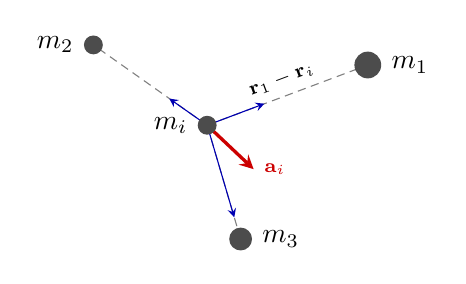
\begin{tikzpicture}[scale=0.85,
          body/.style={circle, fill=black!70, inner sep=0pt},
          sep/.style={densely dashed, gray},
          part/.style={->, >=stealth, blue!70!black},
          total/.style={->, >=stealth, very thick, red!80!black}]
        \coordinate (i) at (0, 0);
        \coordinate (j1) at (2.4, 0.9);
        \coordinate (j2) at (-1.7, 1.2);
        \coordinate (j3) at (0.5, -1.7);

        \draw[sep] (i) -- (j1) node[midway, above, sloped, black, font=\scriptsize] {$\mathbf{r}_1 - \mathbf{r}_i$};
        \draw[sep] (i) -- (j2);
        \draw[sep] (i) -- (j3);

        \draw[part] (i) -- ++(0.855, 0.322);
        \draw[part] (i) -- ++(-0.566, 0.398);
        \draw[part] (i) -- ++(0.405, -1.376);
        \draw[total] (i) -- ++(0.694, -0.656) node[right, font=\scriptsize] {$\mathbf{a}_i$};

        \node[body, minimum size=2.4mm, label={left:$m_i$}] at (i) {};
        \node[body, minimum size=3.4mm, label={right:$m_1$}] at (j1) {};
        \node[body, minimum size=2.4mm, label={left:$m_2$}] at (j2) {};
        \node[body, minimum size=2.9mm, label={right:$m_3$}] at (j3) {};
      \end{tikzpicture}
    \end{column}

    \begin{column}{0.5\textwidth}
      \begin{itemize}
        \item Every particle pulls every other particle towards itself ({\color{blue!70!black}blue}), with a strength $\propto m_j / r^2$.
        \item The acceleration of particle $i$ is the vector sum of all the pulls ({\color{red!80!black}red}):
      \end{itemize}
      \[ \mathbf{a}_i = \sum_{j \neq i} m_j \frac{\mathbf{r}_j - \mathbf{r}_i}{|\mathbf{r}_j - \mathbf{r}_i|^3} \]
      \begin{itemize}
        \item The units are chosen so that $G = 1$.
        \item $N$ particles have $N(N-1)/2$ pairs: 3 for 3 particles, but about 500\,000 for 1000 particles. This is where the time goes.
      \end{itemize}
    \end{column}
  \end{columns}
\end{frame}


\begin{frame}
  \frametitle{From forces to motion}
  \begin{columns}[T]
    \begin{column}{0.58\textwidth}
      \begin{itemize}
        \item The position $\mathbf{r}_i$ and the velocity $\mathbf{v}_i$ of each particle change as
          \[ \frac{d\mathbf{r}_i}{dt} = \mathbf{v}_i, \qquad \frac{d\mathbf{v}_i}{dt} = \mathbf{a}_i(\mathbf{r}_1, \ldots, \mathbf{r}_N). \]
        \item The acceleration of each particle depends on the positions of all the others, so the equations are coupled. For $N \geq 3$, they have no general exact solution.
        \item Instead, we advance the system in small time steps $\Delta t$, short compared with its fastest changes, such as orbital periods and close encounters.
        \item In a long simulation, small errors in each step can add up. A good method keeps them from growing.
      \end{itemize}
    \end{column}

    \begin{column}{0.42\textwidth}
      \centering
      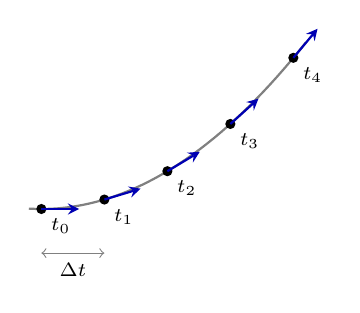
\begin{tikzpicture}[scale=0.8,
          dot/.style={circle, fill=black, inner sep=1.3pt},
          vel/.style={->, >=stealth, blue!70!black, thick}]
        % The true path of one particle
        \draw[gray, thick, domain=-0.2:4.2, samples=40] plot (\x, {0.15*\x*\x});
        % The particle at the start of each time step, with its velocity
        \foreach \x in {0, 1, 2, 3, 4} {
          \node[dot] at (\x, {0.15*\x*\x}) {};
          \draw[vel] (\x, {0.15*\x*\x}) -- ++({0.6/sqrt(1 + (0.3*\x)^2)}, {0.6*0.3*\x/sqrt(1 + (0.3*\x)^2)});
          \node[font=\scriptsize, below right] at (\x, {0.15*\x*\x}) {$t_{\x}$};
        }
        % One time step
        \draw[<->, gray] (0, -0.7) -- node[below, black, font=\scriptsize] {$\Delta t$} (1, -0.7);
      \end{tikzpicture}

      \vspace*{2mm}
      \raggedright
      {\small A trajectory sampled at the times $t_n = n \, \Delta t$. The velocity (blue) changes within each step, and the method must approximate this change.}
    \end{column}
  \end{columns}
\end{frame}


\section{Leapfrog}

\begin{frame}
  \frametitle{The simplest method: Euler}
  \begin{columns}[T]
    \begin{column}{0.48\textwidth}
      \begin{align*}
        \mathbf{r}_{n+1} &= \mathbf{r}_n + \mathbf{v}_n \, \Delta t \\
        \mathbf{v}_{n+1} &= \mathbf{v}_n + \mathbf{a}_n \, \Delta t
      \end{align*}
      \begin{itemize}
        \item $\mathbf{r}_n$ is the position at time $t_n = n \, \Delta t$.
        \item Euler's method uses the velocity and the acceleration at the \emph{start} of the step for the whole step.
        \item Simple, but systematically wrong: on a circular orbit, the planet spirals outwards and finally escapes. A smaller $\Delta t$ only slows this down.
      \end{itemize}
    \end{column}

    \begin{column}{0.52\textwidth}
      \centering
      % Computed: circular orbit with GM = 1 and radius 1, 25 Euler steps
      % with dt = 0.2 (about 31 steps per orbit).
      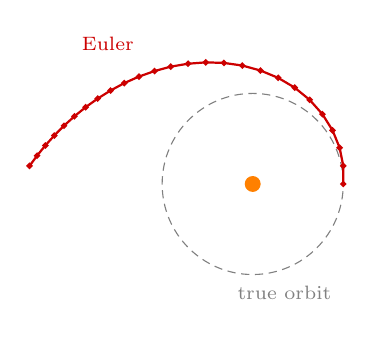
\begin{tikzpicture}[scale=1.15]
        \draw[gray, densely dashed] (0, 0) circle (1);
        \fill[orange] (0, 0) circle (2.5pt);
        \draw[red!80!black, thick] plot[mark=*, mark size=0.6pt] coordinates {(1.000,0.000) (1.000,0.200) (0.960,0.400) (0.882,0.592) (0.770,0.771) (0.629,0.929) (0.464,1.064) (0.281,1.172) (0.086,1.253) (-0.115,1.308) (-0.318,1.337) (-0.518,1.343) (-0.714,1.328) (-0.904,1.296) (-1.084,1.247) (-1.256,1.186) (-1.418,1.114) (-1.570,1.032) (-1.712,0.943) (-1.845,0.848) (-1.969,0.747) (-2.084,0.643) (-2.191,0.535) (-2.290,0.425) (-2.381,0.313) (-2.464,0.200)};
        \node[font=\scriptsize, gray] at (0.35, -1.2) {true orbit};
        \node[font=\scriptsize, red!80!black] at (-1.6, 1.55) {Euler};
      \end{tikzpicture}

      \vspace*{1mm}
      {\scriptsize A circular orbit computed with Euler's method, with about 31 steps per orbit. After 25 steps, the planet is already 2.5 times further from the star.}
    \end{column}
  \end{columns}
\end{frame}


\begin{frame}
  \frametitle{Why Euler goes wrong}
  \begin{columns}[T]
    \begin{column}{0.5\textwidth}
      \centering
      % One step along a circular orbit, moving clockwise from 125 to 55
      % degrees. Both arrows have the length of the true arc, |v| dt.
      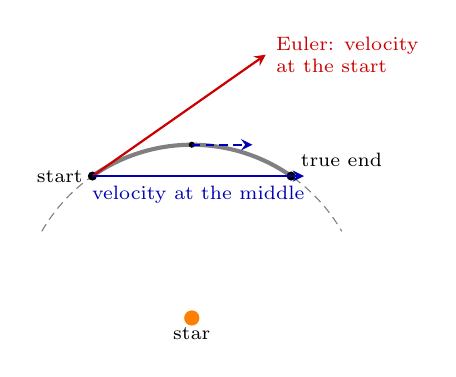
\begin{tikzpicture}[scale=1.1,
          vstart/.style={->, >=stealth, thick, red!80!black},
          vmid/.style={->, >=stealth, thick, blue!70!black}]
        \draw[gray, densely dashed] (150:2) arc (150:30:2);
        \draw[gray, line width=1.5pt] (125:2) arc (125:55:2);
        \fill[orange] (0, 0) circle (2.5pt) node[below, black, font=\scriptsize] {star};
        \fill (125:2) circle (1.5pt) node[left, font=\scriptsize] {start};
        \fill (55:2) circle (1.5pt) node[above right, font=\scriptsize] {true end};
        \fill (90:2) circle (1pt);
        % Euler: the velocity at the start
        \draw[vstart] (125:2) -- ++(35:2.443) node[right, font=\scriptsize, align=left] {Euler: velocity\\at the start};
        % Leapfrog: the velocity at the middle, which is parallel to the chord
        \draw[->, >=stealth, thick, densely dashed, blue!70!black] (90:2) -- ++(0:0.7);
        \draw[vmid] (125:2) -- ++(0:2.443) node[below, pos=0.5, font=\scriptsize, align=center] {velocity at the middle};
      \end{tikzpicture}
    \end{column}

    \begin{column}{0.5\textwidth}
      \begin{itemize}
        \item On an orbit, the velocity turns all the time. The velocity at the start points away from the orbit, so every Euler step lands outside it.
        \item The velocity at the \emph{middle} of the step lands (almost) at the right place.
      \end{itemize}
      \vspace*{2mm}
      \textbf{Lesson:} use the value at the \emph{middle} of the step.
    \end{column}
  \end{columns}
\end{frame}


\begin{frame}
  \frametitle{Leapfrog: positions and velocities take turns}
  \centering
  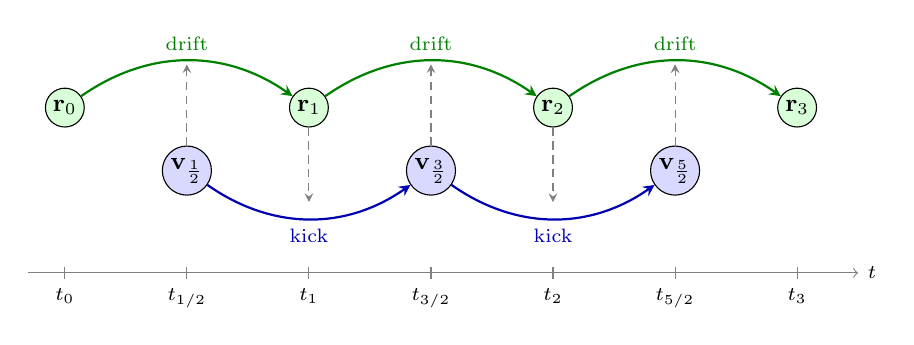
\begin{tikzpicture}[x=1.55cm,
      rnode/.style={circle, draw, fill=green!15, inner sep=1.5pt, font=\small},
      vnode/.style={circle, draw, fill=blue!15, inner sep=1pt, font=\small},
      jump/.style={->, >=stealth, thick},
      uses/.style={->, >=stealth, densely dashed, gray}]
    % Time axis
    \draw[->, gray] (-0.3, -0.5) -- (6.5, -0.5) node[right, black, font=\scriptsize] {$t$};
    \foreach \x/\t in {0/$t_0$, 1/$t_{1/2}$, 2/$t_1$, 3/$t_{3/2}$, 4/$t_2$, 5/$t_{5/2}$, 6/$t_3$}
      \draw[gray] (\x, -0.42) -- (\x, -0.58) node[below, black, font=\scriptsize] {\t};

    % Positions at whole steps, velocities at half steps
    \foreach \k in {0, 1, 2, 3} \node[rnode] (r\k) at (2*\k, 1.6) {$\mathbf{r}_{\k}$};
    \node[vnode] (v0) at (1, 0.8) {$\mathbf{v}_{\frac{1}{2}}$};
    \node[vnode] (v1) at (3, 0.8) {$\mathbf{v}_{\frac{3}{2}}$};
    \node[vnode] (v2) at (5, 0.8) {$\mathbf{v}_{\frac{5}{2}}$};

    % Each one jumps over the other
    \draw[jump, green!50!black] (r0) to[bend left=35] node[above, font=\scriptsize] {drift} (r1);
    \draw[jump, green!50!black] (r1) to[bend left=35] node[above, font=\scriptsize] {drift} (r2);
    \draw[jump, green!50!black] (r2) to[bend left=35] node[above, font=\scriptsize] {drift} (r3);
    \draw[jump, blue!70!black] (v0) to[bend right=35] node[below, font=\scriptsize] {kick} (v1);
    \draw[jump, blue!70!black] (v1) to[bend right=35] node[below, font=\scriptsize] {kick} (v2);

    % ... using the value of the other one from the middle of its jump
    \draw[uses] (v0) -- (1, 2.15);
    \draw[uses] (v1) -- (3, 2.15);
    \draw[uses] (v2) -- (5, 2.15);
    \draw[uses] (r1) -- (2, 0.4);
    \draw[uses] (r2) -- (4, 0.4);
  \end{tikzpicture}

  \vspace*{1mm}
  \begin{columns}[T]
    \begin{column}{0.5\textwidth}
      \begin{itemize}
        \item Positions live at whole steps, velocities at half steps. They jump over each other, like children playing leapfrog.
        \item The dashed arrows show that each jump uses the other quantity from exactly the middle of the jump.
      \end{itemize}
    \end{column}
    \begin{column}{0.5\textwidth}
      \begin{align*}
        \text{drift:} \quad \mathbf{r}_{n+1} &= \mathbf{r}_n + \mathbf{v}_{n+1/2} \, \Delta t \\
        \text{kick:} \quad \mathbf{v}_{n+3/2} &= \mathbf{v}_{n+1/2} + \mathbf{a}_{n+1} \, \Delta t
      \end{align*}
      {\small $\mathbf{a}_{n+1}$ is computed from the positions $\mathbf{r}_{n+1}$.}
    \end{column}
  \end{columns}
\end{frame}


\begin{frame}
  \frametitle{Kick-drift-kick: back to whole steps}
  \begin{columns}[T]
    \begin{column}{0.42\textwidth}
      \begin{itemize}
        \item \textbf{Kick:} change the velocities. Gravity gives the particles a push.
        \item \textbf{Drift:} change the positions. The particles coast with their current velocities.
        \item Velocities at half steps are awkward: the input gives $\mathbf{v}_0$, not $\mathbf{v}_{1/2}$, and the output needs $\mathbf{r}$ and $\mathbf{v}$ at the same times.
        \item Fix: split each kick into two half kicks. Two half kicks in a row are one full kick, so the result is the same leapfrog.
      \end{itemize}
    \end{column}

    \begin{column}{0.58\textwidth}
      \centering
      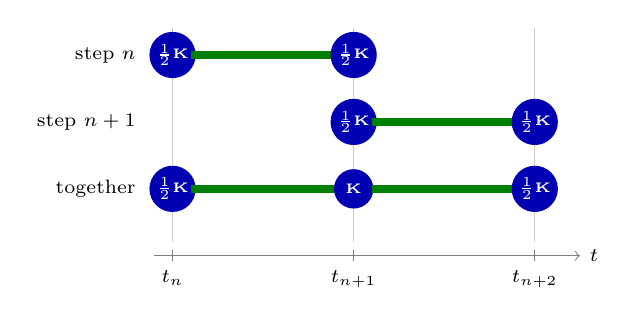
\begin{tikzpicture}[x=2.3cm, y=0.85cm,
          kick/.style={circle, fill=blue!70!black, text=white, inner sep=1pt, font=\tiny\bfseries},
          drift/.style={line width=3pt, green!50!black},
          lab/.style={font=\scriptsize, anchor=east}]
        % Time axis
        \draw[->, gray] (-0.1, 0) -- (2.25, 0) node[right, black, font=\scriptsize] {$t$};
        \foreach \x/\t in {0/$t_n$, 1/$t_{n+1}$, 2/$t_{n+2}$} {
          \draw[gray] (\x, 0.08) -- (\x, -0.08) node[below, black, font=\scriptsize] {\t};
          \draw[gray!40] (\x, 0.2) -- (\x, 3.4);
        }

        % Step n
        \node[lab] at (-0.15, 3) {step $n$};
        \node[kick] at (0, 3) {$\frac{1}{2}$K};
        \draw[drift] (0.1, 3) -- (0.9, 3);
        \node[kick] at (1, 3) {$\frac{1}{2}$K};

        % Step n+1
        \node[lab] at (-0.15, 2) {step $n+1$};
        \node[kick] at (1, 2) {$\frac{1}{2}$K};
        \draw[drift] (1.1, 2) -- (1.9, 2);
        \node[kick] at (2, 2) {$\frac{1}{2}$K};

        % Together
        \node[lab] at (-0.15, 1) {together};
        \node[kick] at (0, 1) {$\frac{1}{2}$K};
        \draw[drift] (0.1, 1) -- (0.9, 1);
        \node[kick, minimum size=5mm] at (1, 1) {K};
        \draw[drift] (1.1, 1) -- (1.9, 1);
        \node[kick] at (2, 1) {$\frac{1}{2}$K};
      \end{tikzpicture}

      \vspace*{2mm}
      {\scriptsize Blue circles: kicks, which happen at one instant. Green bars: drifts, which last a whole step. In the middle, the half kick that ends step $n$ and the half kick that starts step $n+1$ add up to one full kick.}
    \end{column}
  \end{columns}
\end{frame}


% A circled step number for the next frame
\newcommand{\stepnum}[1]{\tikz[baseline=(c.base)]\node[circle, draw, inner sep=0.6pt, font=\tiny] (c) {#1};}

\begin{frame}
  \frametitle{One leapfrog step in detail}
  \begin{columns}[T]
    \begin{column}{0.45\textwidth}
      At the start of step $n$, we know $\mathbf{r}_n$, $\mathbf{v}_n$, and $\mathbf{a}_n$ (from the previous step).

      \vspace*{2mm}
      \begin{tabular}{@{}l@{\hspace{1mm}}l@{\hspace{2mm}}l@{}}
        \stepnum{1} & kick  & $\mathbf{v}_{n+1/2} = \mathbf{v}_n + \mathbf{a}_n \, \Delta t / 2$ \\[1mm]
        \stepnum{2} & drift & $\mathbf{r}_{n+1} = \mathbf{r}_n + \mathbf{v}_{n+1/2} \, \Delta t$ \\[1mm]
        \stepnum{3} & force & $\mathbf{a}_{n+1}$ from the positions $\mathbf{r}_{n+1}$ \\[1mm]
        \stepnum{4} & kick  & $\mathbf{v}_{n+1} = \mathbf{v}_{n+1/2} + \mathbf{a}_{n+1} \, \Delta t / 2$ \\
      \end{tabular}

      \vspace*{3mm}
      \begin{itemize}
        \item $\mathbf{a}_{n+1}$ is reused as $\mathbf{a}_n$ in the next step, so each step computes the forces only once, like Euler.
        \item Step 3 takes almost all the time, so it is the step to parallelise.
      \end{itemize}
    \end{column}

    \begin{column}{0.55\textwidth}
      \centering
      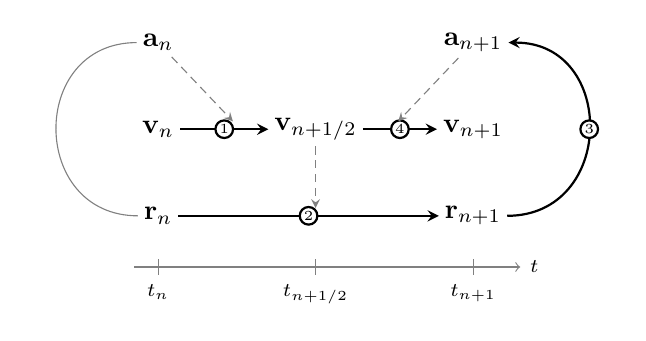
\begin{tikzpicture}[
          state/.style={inner sep=2pt},
          advance/.style={->, >=stealth, thick},
          uses/.style={->, >=stealth, densely dashed, gray},
          num/.style={circle, draw, fill=white, inner sep=0.6pt, font=\tiny}]
        % Accelerations (top), velocities (middle), and positions (bottom)
        \node[state] (a0) at (0, 1.1) {$\mathbf{a}_n$};
        \node[state] (a1) at (4, 1.1) {$\mathbf{a}_{n+1}$};
        \node[state] (v0) at (0, 0) {$\mathbf{v}_n$};
        \node[state] (vh) at (2, 0) {$\mathbf{v}_{n+1/2}$};
        \node[state] (v1) at (4, 0) {$\mathbf{v}_{n+1}$};
        \node[state] (r0) at (0, -1.1) {$\mathbf{r}_n$};
        \node[state] (r1) at (4, -1.1) {$\mathbf{r}_{n+1}$};

        % The four steps
        \draw[advance] (v0) -- node[num] {1} (vh);
        \draw[advance] (r0) -- node[num] {2} (r1);
        \draw[advance] (r1.east) to[out=0, in=0, looseness=1.6] node[num] {3} (a1.east);
        \draw[advance] (vh) -- node[num] {4} (v1);

        % What each step uses; a_n comes from the previous step
        \draw[uses] (a0) -- (0.95, 0.1);
        \draw[uses] (a1) -- (3.05, 0.1);
        \draw[uses] (vh) -- (2, -1.0);
        \draw[gray] (r0.west) to[out=180, in=180, looseness=1.6] (a0.west);

        % Time axis
        \draw[->, gray] (-0.3, -1.75) -- (4.6, -1.75) node[right, black, font=\scriptsize] {$t$};
        \foreach \x/\t in {0/$t_n$, 2/$t_{n+1/2}$, 4/$t_{n+1}$}
          \draw[gray] (\x, -1.65) -- (\x, -1.85) node[below, black, font=\scriptsize] {\t};
      \end{tikzpicture}

      \vspace*{1mm}
      {\scriptsize Solid arrows: the four steps. Dashed arrows: what each step uses.}
    \end{column}
  \end{columns}
\end{frame}


\begin{frame}[fragile]
  \frametitle{Leapfrog in code}
  \begin{columns}[T]
    \begin{column}{0.5\textwidth}
      \begin{lstlisting}
! Accelerations at t = 0
call accelerations(m, r, a)

do step = 1, n_steps
  v = v + a * dt / 2           ! kick
  r = r + v * dt               ! drift
  call accelerations(m, r, a)  ! force
  v = v + a * dt / 2           ! kick
end do
      \end{lstlisting}
      This is the loop in \texttt{leapfrog.f90}, where the force calculation is written out in full instead of being a subroutine.
    \end{column}

    \begin{column}{0.5\textwidth}
      \begin{block}{Choosing $\Delta t$}
        \begin{itemize}
          \item $\Delta t$ must be short compared with the fastest changes in the system, such as close encounters between particles.
          \item Test: run with $\Delta t$ and with $\Delta t / 2$. If the results differ too much, $\Delta t$ is too large.
        \end{itemize}
      \end{block}
      \begin{block}{Testing the code}
        In \texttt{input.dat}, three equal masses chase each other along a figure eight, and return to their starting positions every 6.33 time units. A correct program reproduces this orbit again and again.
      \end{block}
    \end{column}
  \end{columns}
\end{frame}


\section{Tasks}

\begin{frame}
  \frametitle{Exercise 1: modules}
  \begin{enumerate}
    \item Create a module \texttt{geometry} in the file \texttt{geometry.f90} that contains:
      \begin{itemize}
        \item the types \texttt{vector3d} and \texttt{point3d}, both with 64-bit real components \texttt{x}, \texttt{y}, and \texttt{z},
        \item the functions \texttt{sumvp}, \texttt{sumpv}, \texttt{subpv}, \texttt{subpp}, \texttt{mulrv}, \texttt{mulvr}, and \texttt{divvr} for adding a vector to a point, subtracting a vector from a point (a point) or a point from a point (a vector), and multiplying and dividing vectors by reals,
        \item operators that match these functions,
        \item a function \texttt{distance} that returns the distance between two points.
      \end{itemize}
    \item Create a module \texttt{particle} in the file \texttt{particle.f90} that uses the \texttt{geometry} module and contains a type \texttt{particle3d} with the components:
      \begin{itemize}
        \item \texttt{p}, a \texttt{point3d} for the position,
        \item \texttt{v}, a \texttt{vector3d} for the velocity,
        \item \texttt{m}, a real for the mass.
      \end{itemize}
  \end{enumerate}

  \begin{block}{Why two types with the same components?}
    A point is a location (a position). A vector is a displacement (a velocity, an acceleration, or the difference of two points). Point + vector is a point and point $-$ point is a vector, but point + point means nothing. With separate types, the compiler rejects such mistakes.
  \end{block}
\end{frame}


\begin{frame}
  \frametitle{Exercise 1: the program}
  \begin{enumerate}
    \setcounter{enumi}{2}
    \item Change the \texttt{leapfrog.f90} code to use the \texttt{geometry} and \texttt{particle} modules, and store the program in the file \texttt{ex1.f90}.
    \item Read the simulation setup from a file whose name is given as a command-line argument.
    \item Write the simulation data into the file \texttt{output.dat}. Each line contains the state of the simulation at one time as \texttt{t p1x p1y p1z p2x p2y p2z ... pnx pny pnz}.
    \item Write a makefile for the project.
  \end{enumerate}

  \vspace*{3mm}
  Check your program with \texttt{input.dat}: the three bodies should follow the same figure-eight orbit again and again.
\end{frame}


\begin{frame}
  \frametitle{Exercise 1: OpenMP}
  \begin{enumerate}
    \setcounter{enumi}{6}
    \item Parallelise the calculation of the accelerations with OpenMP.
      \begin{itemize}
        \item The program must compile and give the same results both with and without \texttt{-fopenmp}. Add both builds to the makefile.
        \item Hint: the loop over the pairs of particles updates the accelerations of both particles of the pair. What happens if two threads update the same particle at the same time?
      \end{itemize}
    \item Measure how the run time depends on the number of particles and the number of threads.
      \begin{itemize}
        \item Create the initial conditions with \texttt{random\_sphere.f90} for $N$ = 1000, 2000, 5000, and 10\,000. Give it a seed, so that every run uses the same particles.
        \item Run each case with 1, 2, 4, and 8 threads (set \texttt{OMP\_NUM\_THREADS}).
        \item Set \texttt{dt\_out} equal to \texttt{t\_end} while timing, so that writing the output does not dominate.
        \item Report the run times and the speed-ups in a table or a figure in the \texttt{README.md}, and explain what you see.
      \end{itemize}
  \end{enumerate}
\end{frame}


\begin{frame}
  \frametitle{Exercise 1: submission}
  \begin{enumerate}
    \setcounter{enumi}{8}
    \item Write a \texttt{README.md} for the exercise that explains how the code works, how to compile and run it, and the results of the timing study.
    \item Create a pull request (PR) with your code, and add all the course participants as reviewers.
    \item Review the code in the other students' PRs, and write at least one comment on each.
    \item (Optional) Revise your code based on the comments you have received.
    \item In the PR, tag the teacher and say that you have finished the exercise.
  \end{enumerate}
\end{frame}


\begin{frame}
  \frametitle{Exercise 1: scoring}
  \textbf{Scoring} is based on
  \begin{itemize}
    \item Code (80\%)
      \begin{enumerate}
        \item Functionality: the code works as described, also without OpenMP.
        \item Understandability: the code is clear to read and logical.
        \item Comments: all the functionality in the modules and the program is documented with comments.
        \item Use of guidelines: the code uses the type, function, and file names exactly as written in the exercise.
        \item Timing study: the measurements are complete and explained.
      \end{enumerate}
    \item Collaboration (20\%): GitHub PRs, PR comments, and participation.
  \end{itemize}

  \textbf{Bonus points} for anything that goes beyond what has been taught in class, frequent commits, and interaction (asking and answering questions, and so on). If in doubt, ask!

  \vspace*{2mm}
  \textbf{Notes:} Save all the source files in \texttt{students/<initials>/course\_exercise\_1}. All the real variables must be 64-bit. The code should compile without warnings with \texttt{gfortran -Wall}. Commit your changes often, and feel free to work with branches.
\end{frame}


\end{document}
